\chapter{Automatizácia predikcie a porovnanie s ModeRNA}

V tejto kapitole sa budeme venovať ďalšej automatizácii algoritmu, zjednodušeniu predikcie a implementácií. Pripomenieme výsledky bakalárskej práce a predstavíme dáta na ktorých budeme implementované algoritmy testovať. Okrem toho sme náš algoritmus porovnáme s ďalším nástrojom na predikciu RNA štruktúr ModeRNA, ktorý funguje na podobnom princípe ako náš algoritmus, teda na princípe komparatívneho modelovania. Ďalej doplníme funkcionalitu, vďaka ktorej algoritmus nájde vhodnú template štruktúru pre zadaný target. Nakoniec sa pokúsime riešiť datové problémy, ktoré vznikajú vďaka nezhode fasta sekvencií a sekvencií extrahovaných z odpovedajúcich pdb štruktúr. 

\section{Dáta}
Všetky testovacie dáta boli stiahnuté z webu ProteinDataBank \url{https://www.rcsb.org} \cite{PDB00}. Jedná sa o fasta a pdb súbory RNA molekúl, ktoré majú experimentálne získanú terciárnu štruktúru. Celkový počet molekúl je 1158. Fasta súbory sme ešte následne rozdelili podľa identifikátora vlákien \textit{(chain)} (jedna stiahnutá molekula môže obsahovať viacero štruktúr rozdelených do vlákien). Po tomto rozdelení fasta súborov sme získali 2081 sekvencií. Na tieto dáta budeme v práci ďalej odkazovať ako na \textit{databázu štruktúr}.

\indent Pre testovanie algoritmu sme používali všetky stiahnuté štruktúry sekvencie dĺžky 50 a viac nukleotidov. Najprv sme ich rozdelili do priehradok podľa dĺžky (50-100nt, 101-500nt, 500-viac nt). Štruktúry v priehradkách sme následne spárovali každú s každou ako target - template dvojice a tieto dvojice rozdelili do skupín podľa podobnosti a pomeru medzier vzhľadom na zarovnanie. Takto pripravené dáta sme používali pre testovanie algoritmov z tejto práce.


\section{RMSD}
V tejto sekcii si predstavíme mieru, ktorou budeme vyjadrovať presnosť získaných výsledkov. Budeme merať rozdiely medzi experimentálne získanou štruktúrou a nami napredikovanou štruktúrou. Sekvencia oboch štruktúr je rovnaká, na základe čoho je možné učiť vzájomne si odpovedajúce nukleotidy a tiež atómy. Mierou RMSD (root mean square deviation) vyjadrujeme priemerná vzdialenosť medzi dvojicami atómov v zarovnaných terciárnych štruktúrach a vypočíta sa nasledovne:
$$RMSD = \sqrt{ \frac{1}{N} \sum_{i=1}^{N} \delta_i ^ {2}}$$, pričom $\delta$ je vzdialenosť medzi \textit{N} pármi ekvivalentných atómov. Hodnota je vyjadrená  v  jednotke \textit{Ångström (Å)}, ktorá je rovná  $10^{-10}m$. Na zarovnanie a samotný výpočet RMSD používame funkciu align v programe PyMol \cite{PyMOL}.


\section{Implementácia a automatizácia}
V tejto sekcii vysvetlíme, kde je implementácia algoritmu Trooper dostupná a ako sá dá nainštalovať, použiť a porovnáme v nej tiež zmeny v automatizácií oproti stavu z bakalárskej práce.


\indent Pre implementáciu máme vytvorený repozitár na GitHub-e s adresou \url{https://github.com/galvaner/Trooper}. Repozitár obsahuje viacero vetví. 
Najaktuálnejšia je vetva \textit{multiple\_templates}, ktorá obsahuje aktuálny kód. Okrem toho za zmienku stojí vetva \textit{run\_on\_local\_pc}, kde je pripravená testovacia predikcia štruktúry 4QLM\_A.


\indent Pre spustenie treba splniť nasledujúce software-ové požiadavky:
\begin{enumerate}
\item UNIX-ový operačný systém.
\item Nainštalovať software Rosetta \url{https://www.rosettacommons.org/software/license-and-download}.
\item Nainštalovať software Emboss \url{http://emboss.sourceforge.net/what/} (musí byť dostupný z príkazového riadku).
\item Nainštalovať balík VienaRNA \url{https://www.tbi.univie.ac.at/RNA/} pri použití predikcie sekundárnej štruktúry (musí byť dostupný z príkazového riadku).
\item Nainštalovať PyMOL (musí byť dostupný z príkazového riadku).
\item Nainštalovať Python v2.7 (musí byť dostupný z príkazového riadku).
\item Nainštalovať BioPython.
\end{enumerate}


\indent Pre spustenie treba dodať nasledujúce vstupné súbory:
\begin{enumerate}
\item Dodať súbory do priečinka pairs pomenované \textit{60-75s30-45g\_51\_100l.txt}, pričom čísla a písmená môžu byť zmenené. Každý riadok súboru znamená jednu predikciu a skladá sa z názvov target a template štruktúr. Názvy sú oddelené medzerou a zahŕňajú identifikátor vlákna oddelený od mena štruktúry podtržítkom, napríklad: \textit{4QLM\_A.fasta 4QK9\_A.fasta}.
\item Dodať potrebné pdb súbory do priečinka \textit{pdbs}. 
\item Dodať potrebné fasta súbory do priečinka \textit{fastas}.
\item Dodať potrebné súbory obsahujúce sekundárne štruktúry do priečinka \textit{secondary\_structures}.
\end{enumerate}


\indent V pôvodnej implementácii bežala časť algoritmu na OS Windows a časť na UNIX-e. Medzi operačnými systémami bolo treba manuálne kopírovať súbory, čo je zbytočne zdĺhavé. Kvôli tomu sme algoritmus testovali iba na skupine vybraných dát. Upravili sme implementáciu tak, že dokáže bežať na jednom operačnom systéme a z hľadiska obsluhy sa predikcia skladá z nasledujúcich štyroch krokov (spustení štyroch skriptov):
\begin{enumerate}
\item Príprava predikcie pre FARFAR \textit{prepare\_rosetta\_prediction.sh}.
\item Predikcia FARFAR \textit{startFARFAR.sh}.
\item Konverzia a spojenie výsledkov FARFAR do jedného pdb súbora \textit{extract\_pdbs.sh}.
\item Vyhodnotenie predikcie \textit{concat\_pdbs.sh}.
\end{enumerate}

\indent Rozhodli sme sa teda presunúť beh celého algoritmu na unixový systém. Prečo sme sa rozhodli pre Unix a nie Windows? Hlavným dôvodom je možnosť paralelizácie predikcie FARFAR v Metacentre a taktiež fakt, že Rosetta nie je na Windowse podporovaná. Algoritmus bol upravený tak, že pre predikciu stačí dodať vstupné dáta a spustiť jeden skript na prípravu predikcie bodov 1-7 \autoref{3-kostra} (teda až do spustenia FARFAR predikcie). Následne treba spustiť druhý skript, ktorý spustí predikciu FARFAR. Bolo by možné automaticky spustiť tento skript hneď po prvom, avšak v prípade, že by prvá časť skončila s chybami, máme možnosť ju prekontrolovať a nezahltiť tak metacentrum naplánovaním zbytočných taskov. Po dobehnutí predikcie nekonzervovaných úsekov je treba spustiť tretí skript, ktorý konvertuje výstupy FARFAR z internej reprezentácie do pdb súborov, a zároveň ich zmerguje do výslednej štruktúry. Nakoniec v prípade, že v priečinku s experimentálne získanými štruktúrami existuje predikovaná target štruktúra, môžeme spustiť štvrtý skript, ktorý s ňou porovná napredikovanú štruktúru pomocou programu PyMol a výsledok uloží.


\indent V našom prediktore existuje mnoho konfigurovateľných parametrov, ktoré necheme vždy zadávať na vstupe a ani ich nechceme hardcodovať v rôznych scriptoch. Niektoré sa nachádzajú v shell scriptoch a niektoré v python scriptoch. Preto sme vytvorili konfiguračný súbor \url{Predictor/scripts/config.py}, ktorý obsahuje všetky relevantné parametre uložené prehľadne na jendom mieste \autoref{obr04:config}.

\begin{figure}%[p]\centering
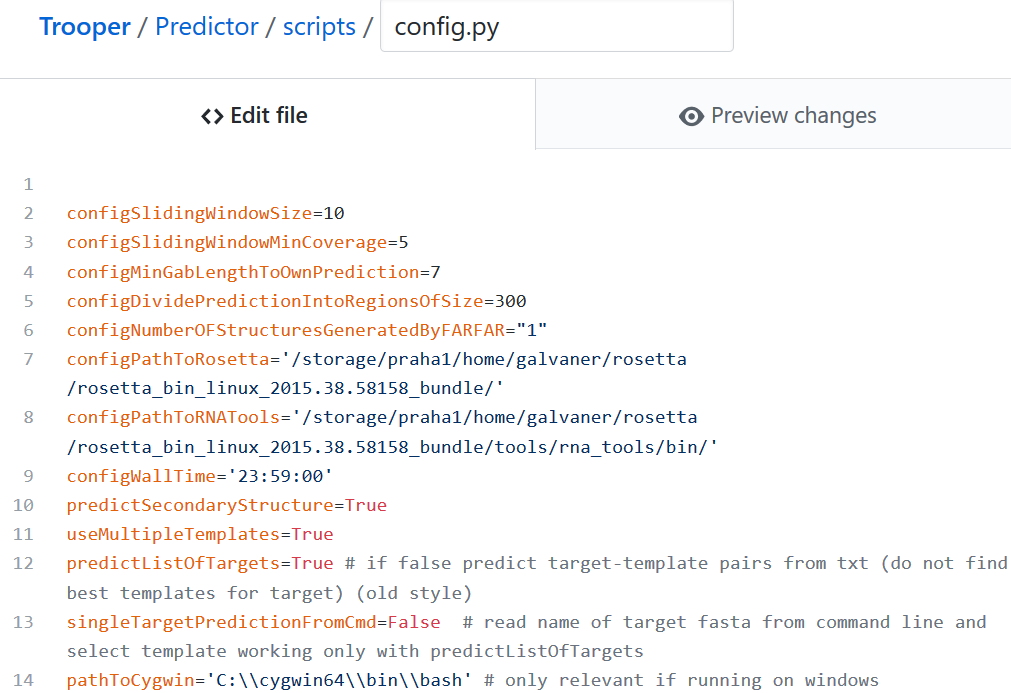
\includegraphics[width=\textwidth]{../img/config}
\caption{Príklad konfiguračného súboru.}
\label{obr04:config}
\end{figure}


%\indent Kroky potrebné vykonať pre kompletnú predikciu štruktúry:
%\begin{enumerate}
%\item Dodať vstupný súbor párov target - template
%\item Uistiť sa, že potrebné pdb a fasta súbory sa nachádzajú v rovnomenných priečinkoch.
%\item Spustiť skript prepare\_rosetta\_prediction.sh a uistiť sa, že dobehol.
%\item Spustiť skript startFARFAR.sh.
%\item Počkať, kým predikcia nekonzervovaných úsekov dobehne.
%\item Spustiť skript extract\_pdbs.sh.
%\item Spustiť skript concat\_pdbs.sh
%\end{enumerate}

\section{Výsledky pôvdného algoritmu}
Pôvodne sme vďaka nedostatočnej automatizácií algoritmu predikovali iba niekoľko náhodne vybraných štruktúr a takto získané výsledky sme prezentovali v bakalárskej práci. Tieto výsledky tu uvedieme kvôli dvom pozorovaniam, ktoré z nich plynú a budú nás zaujímať pri výbere dát pre ďalšie testy v tejto práci.
Prvé pozorovanie ukazuje, že predikovať sekvenciu na základe štruktúry s podobnosťou menšou ako 60\% nie je vhodné, ako vidno aj v tabuľke výsledkov\autoref{tab4.1}. Naopak druhé pozorovanie ukazuje, že pri podobnosti sekvencii väčšej ako 60\% sme schopní dosahovať presnosť predikcie pod 10Å. Tento výsledok je porovnateľný s algoritmom ModeRNA, ako ukážeme v nasledujúcej sekcii. Taktiež je to výrazné zlepšenie oproti de novo algoritmom, kde v článku \cite{Zhao2012} je uvádzaná priemerná RMSD používaných algoritmov pri predikcii štruktúr dĺžky 50-130 nukleotidov približne 20Å. 

\begin{table}[b!]
\centering
\begin{tabular}{cccc}
\toprule
Podobnosť (\%) & Gap (\%)  & Priemer RMSD (Å) & Smerodatná odchýlka  (Å)\\
\midrule
30-45  & 30-45 & 32,05 & 6,09 \\
45-60  & 30-45 & 32,30 & 4,78 \\
60-75  &   0-15 & 11,88 & 7,81 \\
60-75  & 15-30 &   9,63 & 2,33 \\
60-75  & 30-45 &   8,80 & 7,20 \\
75-90  &   0-15 &   6,02 & 4,37 \\
75-90  & 15-30 &   6,93 & 4,45 \\
\bottomrule
\end{tabular}
\caption{Výsledky predikcie pre target template páry dĺžky 50-500 nukleotidov z bakalárskej práce. }\label{tab4.1}
\end{table}


\section{Porovnanie s ModeRNA} \label{ModeRNA}
V bakalárskej práci sme algoritmus porovnávali s algortimom FARFAR, ktorý z princípu nedokáže predikovať príliš dlhé štruktúry \textit{(autori uvádzajú, že FARFAR dosahuje vysokú presnosť len pri štruktúrach veľkosti do 12 nukleotidov)}. Teraz sme sa rozhodli porovnať náš algoritmus s komparatívnou predikciou ModeRNA. Pre porovnanie sme sa rozhodli napredikovať rovnaké sekvencie za pomoci rovnakých target štruktúr a porovnať výsledky z ModeRNA s výsledkami nášho algoritmu. Napísali sme skript \url{ModeRNA/moderRNA.py}, ktorý sa pokúša predikovať target - template páry poskytuté na vstupe. Predikcia v ModeRNA je výrazne rýchlejšia a vytvorenie jednej štruktúry sa väčšinou pohybuje v rádoch minút. Výsledky oboch algoritmov sme porovnali \autoref{tab4.2}, pričom sme uvažovali iba predikcie, ktoré úspešne vytvorili oba algoritmy. V tomto prípade sme rozlišovali dĺžky štruktúr, a to 50-100 nukleotidov a 101-500 nukleotidov. Kritérium na podobnosť tempate štruktúry bolo pre všetky dĺžky rovnaké, a to 60-90\%. Z výsledkov vyplýva, že ModeRNA bola úspešnejšia v predikovaní dlhších štruktúr, pričom naopak náš algoritmus si viedol lepšie pri predikovaní štruktúr kratších. Na druhej strane, ModeRNA dokázala napredikovať celkovo viac štruktúr oproti nášmu algoritmu, pretože dokázala lepšie zvládnuť nedokonalé vstupné dáta. Tieto výsledky sme publikovali v článku \cite{7822808}.

\begin{table}[b!]
\centering
\begin{tabular}{ccc}
\toprule
Dĺžka (nt) & ModeRNA RMSD (Å) & Trooper RMSD (Å) \\
\midrule
50-100    & 5,77 & 8,34  \\
101-500  & 8,25 & 4,29  \\
\bottomrule
50-500  & 6,21 & 7,65  \\
\end{tabular}
\caption{Porovnanie nášho algoritmu s ModeRNA. }\label{tab4.2}
\end{table}

\section{Porovnanie predikcie dlhých štruktúr s ModeRNA}
Algoritmy založené na princípe komparatívneho modelovania majú vďaka vysoko konzervovaným RNA štruktúram potenciál predikovať prakticky neobmedzene dlhé štruktúry, ak pre ne existuje dosť dobrá template štruktúra. Predikcia štruktúr dlhých niekoľko tisic nukleotidov samozrejme prináša problémy, ako napríklad dlhšie nekonzervované úseky a celkovo dlhší čas predikcie. Skúšali sme predikovať 4 rôzne target-template páry aj pomocou nášho algoritmu, aj pomocou ModeRNA algoritmu. Pravdepodobne kvôli tomu, že ModeRNA používa na vyplnenie nekonzervovaných úsekov knižnicu fragmentov, sa v takto dlhej štruktúre našiel nekonzervovaný úsek, ktorý ModeRNA nedokázala napredikovať. Náš algoritmus má síce s dlhými úsekmi problémy tiež, ale vďaka ich de novo predikcii dokázal napredikovať aj takýto úsek \autoref{tab4.3}.

\begin{table}[b!]
\centering
\begin{tabular}{ccccc}
\toprule
Target(len) & Template(len) & Sim(\%) & Trooper & ModeRNA\\
\midrule
3DG0(2904)  & 2O45(2880) & 68  & 13,65 & No fragments candidates.\\
4JI1(1522)  & 4V4Q(1542) & 71,6  & 14,5 &  No fragments candidates.\\
4V6W(1995)  &  4V6X(1869) & 68,3  & 32,7 & Sequences do not match.\\
3DG5(1542)  & 3J2G(1533) &  99,4  & 9,6 & 9,6\\
\bottomrule
\end{tabular}
\caption{Porovnanie výsledkov predikcie vybraných dlhých štruktúr pomocou našeho algoritmu a pomocou ModeRNA. }\label{tab4.3}
\end{table}


\section{Automatické vyhľadanie tempalte štruktúry}
V pôvodnej implementácii  algoritmus očakáva pripravený súbor target a template dvojíc, ktoré bude predikovať. To je vhodné pre účely testovania algoritmu, kedy je našim cieľom zadať vzťah medzi target a template sekvenciou (dĺžka, podobnosť, počet medzier v zarovnaní). V prípade, že by sme našu implementáciu chceli poskytnúť užívateľom tak, aby mohli pomocou nej napredikovať neznámu štruktúru, očakávame, že užívateľ nebude vedieť, akú štruktúru je vhodné použiť ako target. Preto sme naimplementovali možnosť zadať na vstup iba target sekvenciu a náš algoritmus sám určí vhodnú sadu template sekvencií, podľa ktorých by bolo možné cieľovú sekvenciu predikovať čo najlepšie. Počet template sekvencií dodáme algoritmu ako parameter \textit{returnFirstSuitableX} a uživateľovi to dáva teoretickú možnosť napredikovať jeden target podľa viacerých template štruktúr.


\indent Pseudokód algoritmu vyhľadávajúceho template štruktúru:
\lstset{numbers=left, numberstyle=\tiny, stepnumber=1, numbersep=5pt}
\begin{lstlisting}
SelectTemplates(targetSeq, returnFirstSuitableX)
{
   foundSeqs = []
   foreach fastaSeq in allSequences 
   {
       if foundSeqs.Count() == returnFirstSuitable:
	return foundSeqs
       if fastaSeq not usable as template for targetSeq:
          continue
       align := CallEmbossAln(fastaSeq, targetSeq)
       if fastaSeq is better than any of foundSeqs:
          if fastaSeq not too similar to other foundSeqs:
            foundSeq.Add(fastaSeq)
   }		
   return foundSeqs
}
\end{lstlisting}


\indent Algoritmus sme naimplementovali v metóde SelectTemplates a pozostáva z toho, že v cykle postupne globálne zarovnávame target sekvenciu so sekvenciou z databázy sekvencií (v našom prípade zložka s fasta súbormi). Následne  zarovnanie validujeme viacerými validáciami. Najpv validujeme, či vôbec budeme môcť uvažovaný template použiť podľa toho, že neobsahuje príliš veľa neznámych nukleotidov (ak  bol fasta súbor generovaný z pdb, znamená to chýbajúce nukleotidy v pdb). My sme určili minimálny limit 95\% platných nukleotidov. Následne validujeme, podľa samotnej podobnosti target sekvencie a potencionálnej template sekvencie. Nami určený interval podobnosti je v tomto prípade 60\% - 90\% (minimum vychádza z pokusov z bakalárskej práce, maximum je nastavené empiricky tak, aby sa target a template dostatočne líšili). Nakoniec validujeme potencionálnu template sekvenciu medzi už vybranými template sekvenciami. S každou z nich môže mať podobnosť maximálne 90\%. Ak zarovnanie prejde validáciou, štruktúru si označíme ako vhodnú pre predikciu a pokračujeme v cykle. Štruktúru taktiež považujeme za vhodnú ako template iba vtedy, ak  žiadnu veľmi podobnú štruktúru už takto označenú nemáme (podobnosť maximálne 90\%). Ukončovacie kritérium pre cyklus je buď prejdenie všetkých štruktúr a vrátenie požadovaného počtu najlepších, alebo nájdenie prvých \textit{returnFirstSuitableX} štruktúr splňujúce parametre hľadania.


\indent Takto môže užívateľ predikovať štruktúru podľa viacerých odlišných template štruktúr vo viacerých nezávislých predikciách, výsledky potom manuálne porovnať a vybrať ten najlepší. Nevýhodou vyhľadávania vhodných template štruktúr takýmto spôsobom je časová náročnosť, kedy vyhľadanie v našej databáze  môže trvať niekoľko minút, čo je výrazné spomalenie. Takýto problém by bolo možné vyriešiť použitím rýchleho heuristického zarovnania typu BLAST alebo FASTA, no vzhľadom na trvanie predikcie FARFAR a predpokladu, že táto funkcionalita nebude využívaná na hromadnú predikciu štruktúr, sme to nepovažovali za prioritu. Z pohľadu asymptotickej náročnosti platí všetko, čo sme o nej povedali v rozbore v tretej kapitole a okrem toho na začiatok pridáme zložitosť metódy SelectTemplates, ktorá je \textit{O(n$l^2$)}, kde \textit{n} označuje počet štruktúr v databáze a \textit{l} označuje dĺžku štruktúry v databáze. Celková asymtotická zložitosť algoritmu sa teda zvýšila na \textit{O(n$l^2$)}.




\section{Úprava vstupných dát}
V tejto sekcii vysvetlíme chyby objavujúce sa vo vstupných dátach a problémy pre algoritmus z toho plynúce. Následne budeme generovať fasta súbory z pdb súborov preto, aby sme vedeli určiť molekulu nepoužiteľnú pre Trooper a vyhli sa tak problémom, ktoré by nastali neskôr v algoritme počas predikcie.


\indent Fasta a pdb stiahnutéi zo stránok ProteinDataBank sú experimentálne získane štruktúry, ktoré často nie sú kompletné, alebo obsahujú chyby. Problém pre náš algoritmus nastáva hlavne v prípade, kedy sekvencia fasta súboru nesedí so sekvenciou extrahovanou z pdb súboru. Na základe dát, ktorých modifikácia je popísaná v tejto sekcii, sme testovali posledné vylepšenie algoritmu, teda použitie viacerých template štruktúr. Generovanie modifikovaných dát je naimplementované v priečinku s relatívnou cestou Predictor/MyTools/CreateFastasFromPdb.


\indent Principiálne problémy s rozdielnymi sekvenciami v našom algoritme nastávajú v troch konkrétnych prípadoch: 

\begin{enumerate}
\item Pri hľadaní vhodnej template štruktúry pre predikciu (funkcionalita automatického vyhľadávanie template štruktúry).
\item Pri mapovaní temlate štruktúry na konzervované úseky plynúce zo zarovnania sekvencií. \autoref{3-map}
\item Pri hľadaní a mapovaní sekundárných template štruktúr. 
\end{enumerate}

\indent Všetky tri situácie majú rovnakú príčinu a tou je, že algoritmus bude potrebovať namapovať template pdb štruktúru na template fasta sekvenciu. V prípade, že v pdb súbore chýba skupina nukleotidov a zároveň číslovanie nukleotidov oproti fasta súboru nesedí, môže existovať viacero možných mapovaní štruktúry na sekvenciu a my nie sme schopní určiť, ktoré mapovanie je správne.


\indent V prípade že nastane takáto situácia, algoritmus nedokáže pokračovať v predikcii. Doteraz sme to riešili tak, že sme sa pokúsili template fasta sekvenciu posunúť pridaním dummy reziduí na jej začiatok (predpoklad, že z FASTA sekvencie chýba na začiatku pár reziduí a ďalej sa už bude poradie nukleotidov zhodovať s tým v pdb súbore) a v prípade, že sa nám niečo takéto nepodarilo nájsť, danú štruktúru sme ako template nepoužili.


\indent Rozhodli sme sa skúsiť eliminovať tento problém vygenerovaním fasta sekvencie z pdb súborov. Sitáciu nám však komplikuje častá nekompletnosť pdb súborov, kedy sa pravidelne stáva, že začiatok, prípadne koniec štruktúry chýba. Chýbajúce úseky znova nahradzujeme dummy reziduami (písmeno X). Takéto štruktúry môžu byť následne bez problémov použité ako template alebo sekundárny template pri predikcii, pretože pridaný dummy nukleotid X sa nezarovná na target sekvenciu a bude neskôr dopredikovaný. Z princípu sekvencia obsahujúca takéto dummy nukleotidy nemôže byť predikovaná, keďže nevieme, aký nukleotid máme na dané miesto vlastne predikovať.


\indent Okrem problému s mapovaním štruktúry a sekvencie sme riešili aj duplicitu rôzne pomenovaných, ale pritom rovnakých štruktúr. Tomu sme sa v pôvodnej implementácii vyhli, pretože sme si dopredu testovacie dáta rozdelili podľa podobnosti zarovnaní ich sekvencií, a tie sme vzájomne spárovali. Teda ako template sme používali len dosť odlišné template sekvencie od target sekvencie, nakoľko predikovať sekvenciu pomocou inej so skoro 100\% zhodou by bolo triviálne. V prípade, že hľadáme vhodný template, sa však chceme vyhnúť zbytočnému zarovnávaniu sekvencií, a preto si pri generovaní fasta súborov rovno podobné odfiltrujeme. Docielime to jednoducho tak, že pri vygenerovaní novej fasta sekvencie ju globálne zarovnáme na všetky už vygenerované fasta sekvencie, a ak podobnosť presiahne istú konštantnú hranicu (použíli sme 97,5\%), tak takúto sekvenciu nepridáme medzi už vygenerované sekvencie.